\chapter{准备知识}

在对数据立方计算进行研究分析之前,首先介绍一些与数据立方相关的基本知识。本章节主要包括数据立方的定义、数据立方的相关术语、度量函数以及MapReduce的相关知识。

\section{数据立方}
为有效支持 OLAP 应用,Jim Gray 等人于 1996 年提出一种多维数据计算模型 —— 数据立方 (Data Cube) \cite{gray1997data}。该模型是针对事实表中各维度的所有组合对应的聚集计算,即各个维度不同组合的 GroupBy 计算。它利用各个组合之间的关系,提高计算效率。在 OLAP 术语中,聚合属性称为维属性, 被计算的属性称为度量属性。

如图\ref{fact_table_data_cube} 所示,(a) 为事实表 R, A、B、C 为它的维属性,M 为它的度量属性。(b) 为基于事实表 R 构建的数据立方。(b)中的每个视图代表的就是某个特定维属性组合的 GroupBy 结果。所有 GroupBy 结果构成数据立方。

\begin{figure}[!htb]
\centering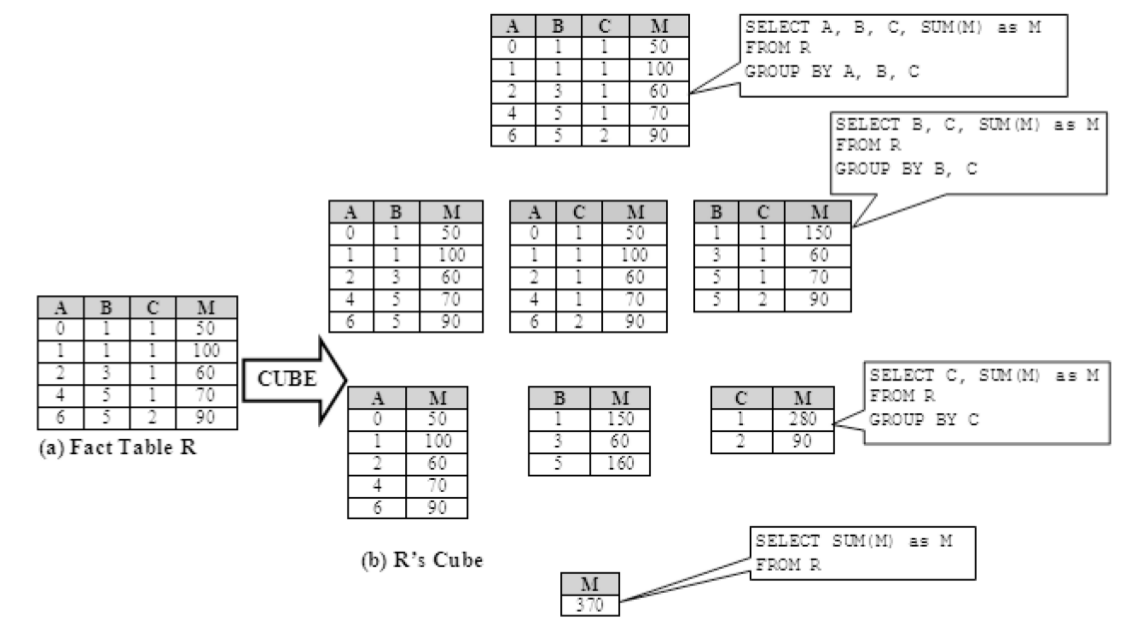
\includegraphics[width=6in]{picture/ch_preliminary/fact_table_data_cube} 
\caption{事实表与数据立方}\label{fact_table_data_cube} 
\end{figure} 

\section{Lattice, Region, Group}

对于图\ref{fact_table_data_cube} 中的所有GroupBy,可用另一种方式表示,如图\ref{abc_lattice} 所示,这种结构称为 Lattice。

\begin{figure}[!htb]
\centering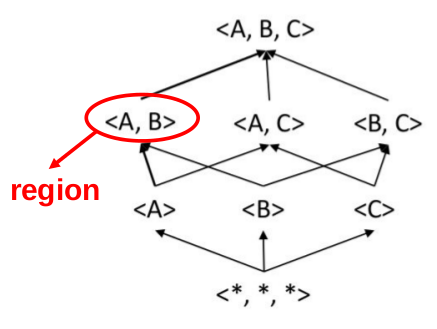
\includegraphics[width=2in]{picture/ch_preliminary/abc_lattice} 
\caption{ABC Lattice}\label{abc_lattice} 
\end{figure} 

在这个lattice中,有维属性组合对应的所有 GroupBy 类型,每个节点表示一种 GroupBy 类型。在lattice中的每个节点称为一个region,也就是一种 GroupBy 类型。箭头连接的两个节点表示它们有父子关系。例如Region(AB)与Region(A)之间有箭头连接,Region(AB)为父,Region(A)为子,表示GroupBy(A)的结果可从GroupBy(AB)的结果计算获得。

一个 region 内有多个 group。group 指的是一个
region中带有具体值的 GroupBy。例如图\ref{fact_table_data_cube} 中的 GroupBy(A),就有表\ref{groupby_a_table}的结果。

\begin{table}[!ht]
\begin{center}
\begin{tabular}{|c|c|}
\hline 
A & M \\ 
\hline 
0 & 50 \\ 
\hline 
1 & 100 \\ 
\hline 
2 & 60 \\ 
\hline 
4 & 70 \\ 
\hline 
6 & 90 \\ 
\hline 
\end{tabular} 
\end{center}
\caption{GroupBy(A)}\label{groupby_a_table}
\end{table}

在表\ref{groupby_a_table}中,Region(A) 中有5个Group,分别是Group(A=0), Group(A=1), Group(A=2), Group(A=4), Group(A=6)。

从lattice中可见,当一个事实表有 D 个维属性时,它对应的数据立方就会有${2}^{D}$个region,也即有 ${2}^{D}$ 种不同类型的 GroupBy 的查询。最简单直接(Naive)的数据立方实现方法,会对每个region进行独立计算并把结果存储起来。对于一张事实表,随着他的维属性数量的增加,它相对应的数据立方的计算与存储代价就会呈指数增长。于是,在 OLAP 中,如何从立方计算、立方存储这两个角度高效地实现数据立方已成为业界内广泛讨论的一个研究课题。


\section{度量}

度量,即对GroupBy的多条数据进行聚合计算,例如SUM,AVG,MEDIAN等。

度量函数一般分为三大类, 分别是分布式度量(Distributive),代数度量(Algebraic)和整体性度量(Holistic)。

以下使用一个二维的数据集$\left\{ {X}_{ij}|i=1,...I; j=1,...J \right\}$分别说明这三种度量函数的区别。

\begin{itemize}

\item \textbf{分布式度量}

对于分布式度量函数 F(),如果存在一个辅助函数 G() 能令 $F(\text\{ {X}_{i,j} \text\}) = G(\text\{ F(\text\{ {X}_{i,j}|i=1,...,I \text\})|j=1,...J \text\})$,则度量函数 F() 为分布式度量函数。常见的分布式度量函数有 COUNT(), MIN(), MAX(), SUM()。大部分分布式度量函数中 $F=G$,但COUNT() 除外。在COUNT()度量函数中,$G=SUM()$。

\item \textbf{代数度量}

对于代数度量函数 F(),如果存在辅助两个函数 G() 和 H(),其中 G() 的输出结果是固定数量的 M 条记录,并且满足$F(\text\{ {X}_{i,j} \text\}) = H(\text\{ G(\text\{ {X}_{i,j}|i=1,...,I \text\})|j=1,...J \text\})$。常见的代数度量函数有AVG(),MaxN(),MinN(),标准差等。例如对于AVG(),函数G()的输出是子集的和以及数量,H()函数则把将各个子集的和相加再除以数量的总和。代数度量的关键是,函数G()的输出结果的数据量是固定的。例如AVG(),无论数据怎么划分,函数G()的输出都是两个值,一个是和,另一个是数量。

\item \textbf{整体性度量}

对于整体性性度量函数 F(),其中间结果,即各个子集的计算结果的数据量大小是不确定的。常见的整体性度量有Median(), Mode(), RANK(), DISTINCT()等。例如使用 DISTINCT()计算一个数列中出现多少不同的数值。若将该数列随意划分,那么每个子数列输出的中间结果仍可能是一个列表,该列表记录了子数列出现哪些数值,即将重复的数值去除。然后再对这些中间结果计算 DISTINCT()。在最坏的情况下,每个子数列输出的中间结果可能就是它本身,因为无重复的数值。

\end{itemize}

之所以要对度量函数进行分类是因为其会影响数据的划分以及数据立方的计算。论文研究的是环境是分布式,因此数据划分是必然的。对于以上三种度量,在分布式度量与代数度量下,数据无论如何划分,使用辅助函数都能计算出最终结果,并且中间结果的数据量是确定的。但对于整体性度量,数据无法随意划分,或者数据的随意划分对其计算的意义并不大,因为中间结果数据量的不确定。然而这并不代表数据不能划分。在后面的章节中会提到,对于整体性度量按照一定的方法对数据进行划分,也能令中间结果的数据大小是确定的。为了方便,在之后的阐述中,将分布式度量与代数度量都归为代数度量。

\section{MapReduce}

MapReduce是Google提出的一个分布式计算架构,用于大规模数据集的并行计算。它被分为Map和Reduce两大阶段。MapReduce的数据流动如图 \ref{mr_data_flow} 所示。它的整个执行流程分为以下几个步骤:

\begin{enumerate}
\item 输入的数据被划分成块分派到各个Map任务中。
\item Map对输入的数据块处理后,以键值对(Key-Value)的格式输出,排序并写到磁盘上。也就是图中的 Sort and spills to disk 阶段。
\item 在Merge阶段从各个Mapper的输出中获取具有相同Key值的数据。
\item 在Sort阶段,将上一阶段阶段合并的结果排序后发到对应的Reducer上。
\item Reducer对输入的键值对进行处理后输出。具有相同Key值的数据会被分派到同一个Reduce函数中。
\end{enumerate}

\begin{figure}[h]
\centering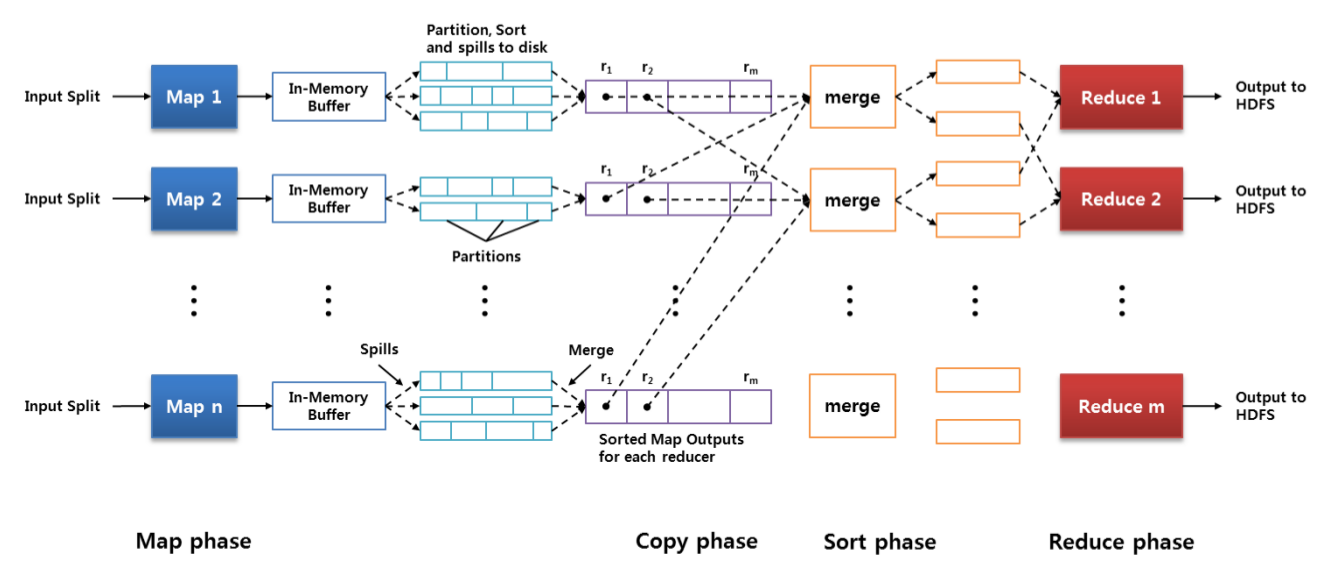
\includegraphics[width=6in]{picture/ch_preliminary/mr_data_flow} 
\caption{MapReduce的数据流动}\label{mr_data_flow} 
\end{figure} 

图\ref{mr_word_count}是用MapReduce进行单词统计的例子。输入的单词被划分成多个块分发到 mapper 上,mapper对于输入的单词逐个输出。在reduce阶段,相同的单词会分派到同一个reducer上,从而统计单词个数。

\begin{figure}[!ht]
\centering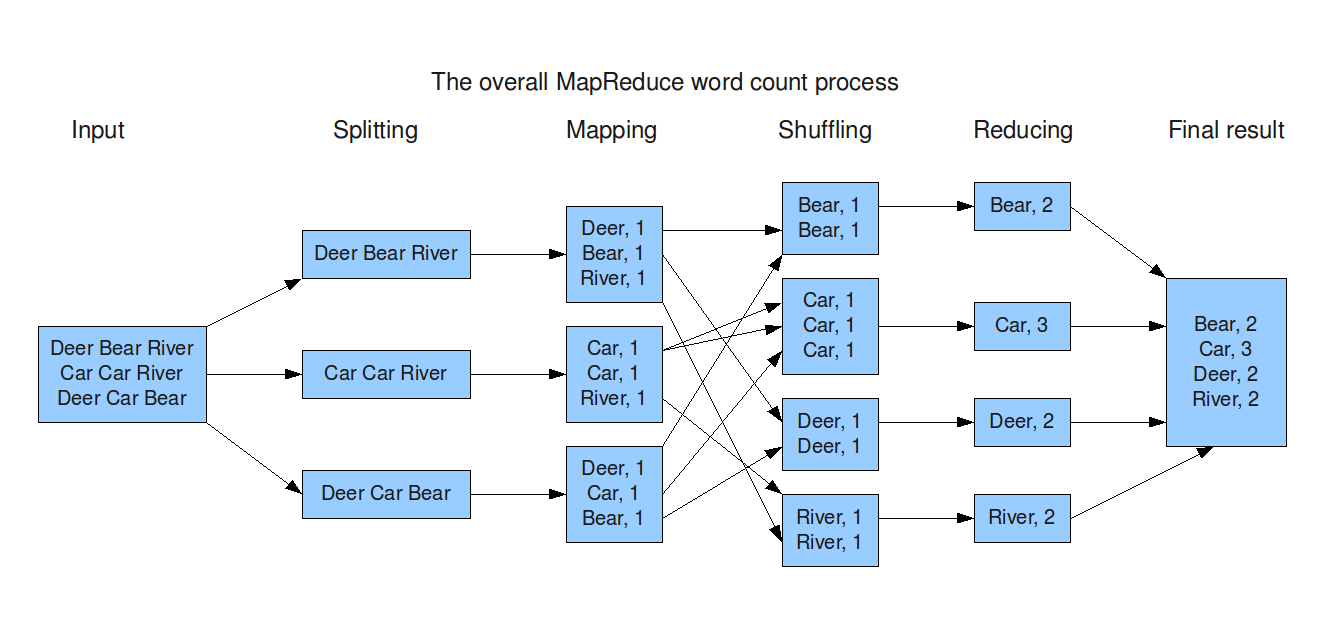
\includegraphics[width=6in]{picture/ch_preliminary/mr_word_count} 
\caption{MapReduce单词统计例子}\label{mr_word_count} 
\end{figure} 

以上仅是MapReduce最基础的机制,为了性能的优化以及用户的需求,MapReduce提供了更多高效、灵活的机制。以下介绍的一些机制在分布式数据立方计算中均会用到。正因为这些机制,令数据立方的计算与MapReduce有更好地结合,从而提高了数据立方的计算效率。

\begin{itemize}

\item Combiner

Combiner等同于本地的reducer,它会对各个 mapper 的输出进行一次本地的 reduce 计算,然后再将数据发到相应的 reducer 上,这样可以减少网络传输的数据量和reducer 的计算量。默认的MapReduce中是没有combiner的,需要用户自定义。

\item Partitioner

具有相同key值的键值对会被分发到同一个reducer上,MapReduce有默认的哈希函数决定不同key值的键值对会被分派到哪个reducer上。但用户可重载Partitioner,自行规定数据的分派。因此可指定不同key值的键值对的分派。

\item GroupPartitioner

在同一个reducer中,一般有多种不同key值的键值对,只有相同key值的数据才会被放在同一个reduce函数中计算。但用户可重载GroupPartitioner,自行规定在同一个reducer中,什么数据需要放在同一个reduce函数中计算,即使它们的key值不同。

\end{itemize}




\section{TeraSort}

TeraSort\cite{o2008terabyte} 的思想在\cite{o2008terabyte} 被用于计算GroupBy,受\cite{o2008terabyte} 的启发,TeraSort被运用于 TSP-Cube 中进行数据立方的计算,因此这里对TeraSort进行简单的介绍。

TeraSort最初用于在 MapReduce 中对全局数据进行排序。虽然 MapReduce 输出的最终结果是有序的,但仅是每个 reducer 输出的数据是有序的,而 reducer 之间的数据是无序的。图\ref{tera_sort}为不使用 TeraSort 与使用 TeraSort 的情况下对原数据使用 MapReduce 排序的结果。图中每个矩形内的数据表示 每个 reducer 的输出。对于不使用 TeraSort 的MapReduce,每个 reducer 输出的数据都是有序的,但是reducer 之间的数据是无序的。而对于使用 TeraSort 的 MapReduce,不仅仅是每个 reducer 内的数据是有序的,reducer 之间的数据也是有序的。

\begin{figure}[ht] 
\centering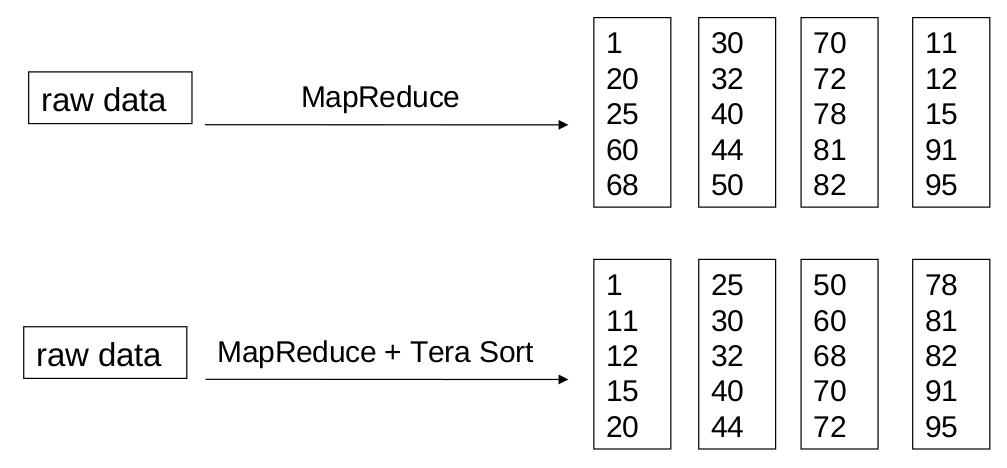
\includegraphics[width=4.5in]{picture/ch_terasort_mr/tera_sort} 
\caption{使用MapReduce+TeraSort对数据排序}\label{tera_sort} 
\end{figure}

TeraSort 能令全局有序的重要关键是,控制落到每个 reducer 上的数据的数据范围。也就是规定某一个范围内的数据必须落在指定的 reducer 上,而不是使用 MapReduce 本身的哈希函数将这些数据随机分发到各个 reducer 上。对于如何确定这些范围值与 reducer 之间的关系,TeraSort 使用采样的方法。

对原数据进行一定比例的采样,这个最佳比例 \cite{tao2013minimal} 已给出证明。将采样的数据都发到同一个 reducer 上。根据 MapReduce 的特性,同一个 reducer 内的数据会被排序。若采样的样本大小为 s,reducer 的数量为 t。那么要从采样序列中选取 t-1 个点作为分界点,这些分界点是限定落入各个 reducer 中的数据的数据范围。对于第 i 个分界点选取的方法是,选取采样序列中的第 $i\times \left \lceil \frac{s}{t} \right \rceil$ 个点作为第 i 个分界点。图 \ref{tera_sort_mr1} 为  TeraSort 采样以及选取分界点的过程。图中假设 reducer 数据量为4,因此选取的分界点数量为3,红色的数字表示其被选为分界点。图中选取了3个分界点,分别为25、50、78,这就给出了4个 reducer 接收数据的数据范围,分别是$\left[- \infty, 25 \right], \left(25, 50 \right], \left(50, 78 \right], \left(78, +\infty \right]$。

\begin{figure}[!htb] 
\centering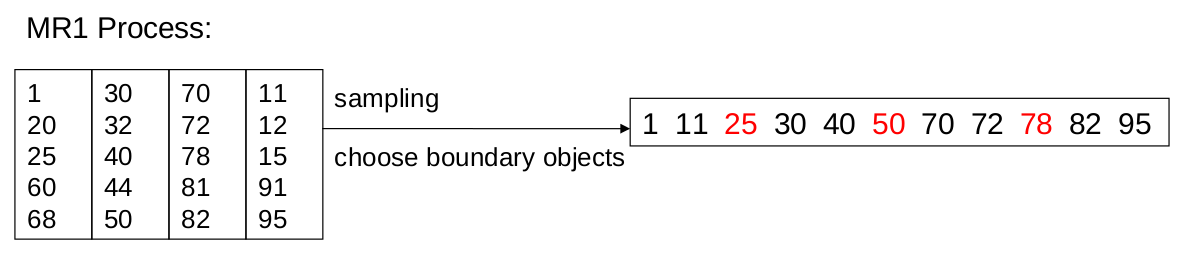
\includegraphics[width=6in]{picture/ch_terasort_mr/tera_sort_mr1} 
\caption{Tera Sort 采样与选取分界点}\label{tera_sort_mr1} 
\end{figure}

以上是第一轮 MapReduce,主要工作是采样以及选取分界点。这些分界点的作用是规定数据必须根据不同的范围落入既定的 reducer 上。在第二轮的 MapReduce 中,对于 Mapper 输出的每一条键值对,根据 key 的值,可使用二分查找等方法(Hadoop中使用Trie树)确定每一条键值对需要分发到的 reducer。最终 MapReduce 的结果就能全局有序。因此这里需要两轮 MapReduce。
